% Respaldo de la figura vectorial sustituida por la imagen aportada.
\begin{figuraNativa}[!ht]{Recorrido general de aseguramiento de calidad. Fuente: elaboración propia}{9-proceso-calidad}
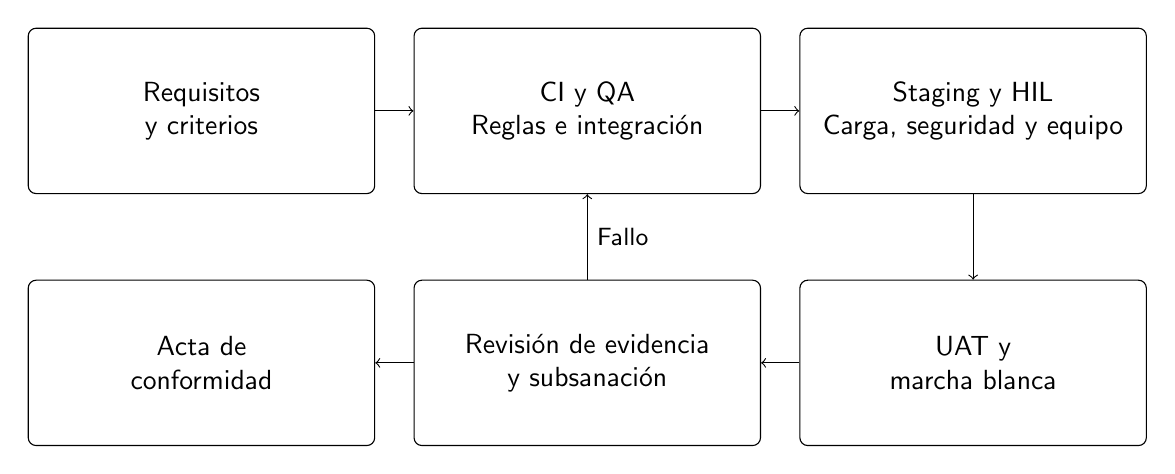
\begin{tikzpicture}[x=1mm,y=1mm,every node/.style={font=\fontsize{10}{12}\selectfont\sffamily,align=center},bloque/.style={draw,rounded corners=1mm,text width=40mm,minimum height=21mm,inner sep=2mm}]
\node[bloque] (r) at (0,0) {Requisitos\\y criterios};
\node[bloque] (u) at (49,0) {CI y QA\\Reglas e integración};
\node[bloque] (h) at (98,0) {Staging y HIL\\Carga, seguridad y equipo};
\node[bloque] (a) at (98,-32) {UAT y\\marcha blanca};
\node[bloque] (e) at (49,-32) {Revisión de evidencia\\y subsanación};
\node[bloque] (c) at (0,-32) {Acta de\\conformidad};
\draw[->] (r)--(u);\draw[->] (u)--(h);\draw[->] (h)--(a);\draw[->] (a)--(e);\draw[->] (e)--(c);
\draw[->] (e)--node[right,font=\fontsize{9}{11}\selectfont\sffamily]{Fallo}(u);
\end{tikzpicture}
\end{figuraNativa}
